\documentclass{beamer}

\usepackage{etex}                     % increase registry size to prevent "No Room for new ..." problems 
                                      % load directly after documentclass

%% setup language
\usepackage[utf8]{inputenc}           % we want the source in utf8
\usepackage[english]{babel}           % select the language to be used (not repsected by siunitx) 

%% setup fonts
\usepackage[T1]{fontenc}              % use T1 fonts (render nicer on screen)
\usepackage{helvet}                   % use Helvetica as sans-serif font

%% setup graphics
% \graphicspath{{../tex/},{img/}}
\DeclareGraphicsExtensions{.pdf,.png,.jpg}

\usepackage{tikz}                     % THE tool for drawing
                                      % Manual: `texdoc pgf` (pgfmanual.pdf)
\usetikzlibrary{backgrounds}          % load backgrounds for Tikz (see manual, Section 25)
\usepgflibrary{arrows.meta}
\usetikzlibrary{bending} 
 
%% use siunitx for simplyfied unit formating
%% replace by experiments official style-file if available
%% 2012-01: asymmetric and multiple uncertainties are not supported
\usepackage{siunitx}
\sisetup{
  separate-uncertainty = true,        % mark uncertainty with \pm
  range-units  = single,              % for range: show unit only once
  range-phrase = { - }                % for range: separate values by -
}

\usepackage{fancyvrb}                 % allow for colored verbatim and other fancy tricks 
\usepackage{minted}                   % for colored code-listings
% \usepackage[super]{nth}               % for 2^{nd} and friends 
\usepackage{soul}

%% define slide layout
%% size of slide: (128 x 96 mm)
\usepackage{appendixnumberbeamer}     % do not count pages in appendix for totalframenumber

%% define helpfull macros

%% create title frame for new section
\newcommand{\sectiontitle}{\begin{frame}{}    
\centering % empty line before \end{frame} necesarry!
{\usebeamercolor[fg]{title} \Huge\insertsection}

\end{frame}}
%% automatically add title slide for new sections
%%   \shortsec is necessary to pass the optional argument on
% \let\oldsection\section
% \renewcommand{\section}[2][\shortsec]{\def\shortsec{#2}\oldsection[#1]{#2}\sectiontitle}

% \usepackage{minted}
% \usemintedstyle{solarized}
\newmintedfile{py}{fontsize=\footnotesize, xleftmargin=12pt}
\newmintedfile{pycon}{fontsize=\footnotesize, xleftmargin=12pt}
\newmintedfile{console}{fontsize=\footnotesize, xleftmargin=12pt}

\newminted{py}{fontsize=\footnotesize, xleftmargin=12pt}
\newminted{pycon}{fontsize=\footnotesize, xleftmargin=12pt}
\newminted{console}{fontsize=\footnotesize, xleftmargin=12pt}

\mode<presentation>
{

  %% Frame Head
  \setbeamertemplate{headline}
  {
	%% first header row: Author, date and frame number
    \begin{beamercolorbox}{section in head/foot}
       \vskip2mm \hspace*{2mm} \insertauthor, \insertshortdate {}{\hfill\insertframenumber{} / \inserttotalframenumber \hspace*{2mm}}\vskip2pt
    \end{beamercolorbox}
    %% seperator line
    \begin{beamercolorbox}[ht=0.1ex]{fg=white,bg=white}
    \end{beamercolorbox}
    %% second header row: sections
    \begin{beamercolorbox}[ht=2.5ex,dp=1.125ex]{section in head/foot}
        \insertsectionnavigationhorizontal{1\paperwidth}{}{}
    \end{beamercolorbox}
  }
  \setbeamercolor{section in head/foot}{fg=white,bg=black}

  %% General Settings
  \setbeamersize{text margin left=0.5cm}
  \setbeamersize{text margin right=0.5cm}


  \setbeamercovered{transparent=25}                  % not active overlays are 25% colored
  \setbeamercolor{alerted text}{fg=red}              % set color for \alert

  \setbeamertemplate{background canvas}{}            % set background to transparent 
%   \setbeamertemplate{background}[grid][step=0.5cm]   % activate grid to help positioning content (decativate before final compile)
}

\addtobeamertemplate{block begin}{}{\vspace*{-2.5mm}}
\addtobeamertemplate{block example begin}{}{\vspace*{-2.5mm}}

% \usefonttheme{structurebold}
% make links like in solarized
\definecolor{base03}{RGB}{0,43,54}
\definecolor{base02}{RGB}{7,54,66}
\definecolor{base01}{RGB}{88,110,117}
\definecolor{base00}{RGB}{101,123,131}
\definecolor{base0}{RGB}{131,148,150}
\definecolor{base1}{RGB}{147,161,161}
\definecolor{base2}{RGB}{238,232,213}
\definecolor{base3}{RGB}{253,246,227}
\definecolor{bgGrey}{RGB}{240,240,240}

\hypersetup{colorlinks=true, linkcolor=blue, urlcolor=blue}
\usecolortheme[named=blue]{structure}
% \setbeamercolor{example}{fg=green}
% \setbeamercolor{block title example}{fg=green, bg=bgGrey}
\setbeamercolor{block title}{bg=bgGrey}
\setbeamercolor{block body}{bg=bgGrey}
\setbeamercolor{block title example}{bg=bgGrey}
\setbeamercolor{block body example}{bg=bgGrey}
% \setbeamertemplate{blocks}[shadow=true]

%%%%%%%%%%%%%%%%%%%%%%%%%%%%%%%%%%%%%%%%%%%%%%%%%%%%%%%%%%%%%%%%
%% ccBeamer 0.1, 2007-07-02                                   %%
%% Written by Sebastian Pipping <webmaster@hartwork.org>      %%
%% ---------------------------------------------------------- %%
%% Licensed under Creative Commons Attribution-ShareAlike 3.0 %%
%% http://creativecommons.org/licenses/by-sa/3.0/             %%
%%%%%%%%%%%%%%%%%%%%%%%%%%%%%%%%%%%%%%%%%%%%%%%%%%%%%%%%%%%%%%%%


%% Images
\newcommand{\CcImageBy}[1]{%
	
\includegraphics[scale=#1]{creative_commons/cc_by_30.pdf}%
}
\newcommand{\CcImageCc}[1]{%
	
\includegraphics[scale=#1]{creative_commons/cc_cc_30.pdf}%
}
\newcommand{\CcImageDevNations}[1]{%
	
\includegraphics[scale=#1]{creative_commons/cc_dev_nations_30.pdf}%
}
\newcommand{\CcImageNc}[1]{%
	
\includegraphics[scale=#1]{creative_commons/cc_nc_30.pdf}%
}
\newcommand{\CcImageNd}[1]{%
	
\includegraphics[scale=#1]{creative_commons/cc_nd_30.pdf}%
}
\newcommand{\CcImagePd}[1]{%
	
\includegraphics[scale=#1]{creative_commons/cc_pd_30.pdf}%
}
\newcommand{\CcImageSa}[1]{%
	
\includegraphics[scale=#1]{creative_commons/cc_sa_30.pdf}%
}
\newcommand{\CcImageSampling}[1]{%
	
\includegraphics[scale=#1]{creative_commons/cc_sampling_30.pdf}%
}
\newcommand{\CcImageSamplingPlus}[1]{%
	
\includegraphics[scale=#1]{creative_commons/cc_sampling_plus_30.pdf}%
}


%% Groups
\newcommand{\CcGroupBy}[1]{% zoom
	\CcImageBy{#1}%
}
\newcommand{\CcGroupByNc}[2]{% zoom, gap
	\CcImageBy{#1}\hspace*{#2}\CcImageNc{#1}%
}
\newcommand{\CcGroupByNcNd}[2]{% zoom, gap
	\CcImageBy{#1}\hspace*{#2}\CcImageNc{#1}\hspace*{#2}\CcImageNd{#1}%
}
\newcommand{\CcGroupByNcSa}[2]{% zoom, gap
	\CcImageBy{#1}\hspace*{#2}\CcImageNc{#1}\hspace*{#2}\CcImageSa{#1}%
}
\newcommand{\CcGroupByNd}[2]{% zoom, gap
	\CcImageBy{#1}\hspace*{#2}\CcImageNd{#1}%
}
\newcommand{\CcGroupBySa}[2]{% zoom, gap
	\CcImageBy{#1}\hspace*{#2}\CcImageSa{#1}%
}
\newcommand{\CcGroupDevNations}[1]{% zoom
	\CcImageDevNations{#1}%
}
\newcommand{\CcGroupNcSampling}[2]{% zoom, gap
	\CcImageNc{#1}\hspace*{#2}\CcImageSampling{#1}%
}
\newcommand{\CcGroupPd}[1]{% zoom
	\CcImagePd{#1}%
}
\newcommand{\CcGroupSampling}[1]{% zoom
	\CcImageSampling{#1}%
}
\newcommand{\CcGroupSamplingPlus}[1]{% zoom
	\CcImageSamplingPlus{#1}%
}


%% Text
\newcommand{\CcLongnameBy}{Attribution}
\newcommand{\CcLongnameByNc}{Attribution-NonCommercial}
\newcommand{\CcLongnameByNcNd}{Attribution-NoDerivs}
\newcommand{\CcLongnameByNcSa}{Attribution-NonCommercial-ShareAlike}
\newcommand{\CcLongnameByNd}{Attribution-NoDerivs}
\newcommand{\CcLongnameBySa}{Attribution-ShareAlike}

\newcommand{\CcNote}[1]{% longname
	This work is licensed under the \textit{Creative Commons #1 3.0 License}.%
}


\newcommand{\git}{git\xspace}
\usepackage{listings}
\usepackage{xspace}
\definecolor{grey}{rgb}{0.5,0.5,0.5}
\usetikzlibrary{graphs}

\title{\git Tutorial}
\author{Nicola Chiapolini}
\institute{Physik-Institut\\
University of Zurich}
\date{\today}
\subject{Python School}

% \AtBeginSection[]
% {
%   \begin{frame}<beamer>{Outline}
%     \tableofcontents[currentsection,currentsubsection]
%   \end{frame}
% }

% create counter for slide number (needed to debug overlays)
\makeatletter\def\c@slideinframe{\beamer@slideinframe}\makeatother
\begin{document}

\lstset{language=bash}

\begin{frame}
  \titlepage

  \begin{center}
    \tiny{Based on talk by Emanuele Olivetti}
    \hspace{1em}
    \tiny\url{https://github.com/emanuele/introduction_to_Git.git}
    \begin{tabular}[t]{lr}
        \mbox{\href{https://creativecommons.org/licenses/bysa/3.0/}
          {\CcGroupBySa{0.35}{0.95ex}}}
        &
        \parbox[b]{8cm}{{\tiny
            \href{https://creativecommons.org/licenses/bysa/3.0/}
            {\CcNote{\CcLongnameBySa}}}} \\
    \end{tabular}
  \end{center}
\end{frame}

% -------------------------------------

\section{Introduction}

\begin{frame}
 \frametitle{Motivation to use Version Control}

\begin{block}{Problem 1}
\vspace*{2.5mm}
``Help!  my code worked yesterday, but I can't recall what I changed.''
\end{block}
\begin{itemize}
  \item track modifications
  \item access old version
\end{itemize}

\vspace*{5mm}
\begin{block}{Problem 2}
\vspace*{2.5mm}
``We would like to work together, but we don't know how!''
\end{block}
\begin{itemize}
  \item concurrent editing
  \item merging
  \item development versions
\end{itemize}
  
\end{frame}

% -------------------------------------

\begin{frame}<1-2>[label=outline]
 \frametitle{Outline}

\only<1>{\tableofcontents}
\only<2->{\tableofcontents[currentsection,currentsubsection]}
  
\end{frame}

% -------------------------------------

\begin{frame}{Survey: Version Control}
\begin{itemize}\setlength{\itemsep}{+3mm}
  \item<alert@+> Q1: Have you heard about \emph{version control}?
  \item<alert@+> Q2: Do you use a version control software (cvs, svn, hg, bzr, git)?
  \item<alert@+> Q3: How much experience do you have with \git?
\end{itemize}
\end{frame}

% -------------------------------------

\begin{frame}
 \frametitle{Uses for \git}

\begin{block}{}
``\emph{Version control} is a system that records changes to a file or set of files over time so that you can recall specific versions later.''\\
\hfill-- Git Website
\end{block}

\begin{itemize}
  \item checkpoints/backups/releases
  \item document developer effort
  \item collaboration across the globe
\end{itemize}

\begin{itemize}
  \item for anything that's text
\begin{itemize}
  \item code
  \item thesis/papers
  \item system config files {\footnotesize (\href{https://github.com/RichiH/vcsh}{vcsh})}
\end{itemize}
 \item ...and everything else {\footnotesize(
    \href{http://penta.debconf.org/dc13_schedule/events/1025.en.html}{"gitify your life"}, 
    \href{https://git-annex.branchable.com/}{git-annex}
    )}
\end{itemize}

\end{frame}

% -------------------------------------

\begin{frame}{Version Control: Local}
\centering
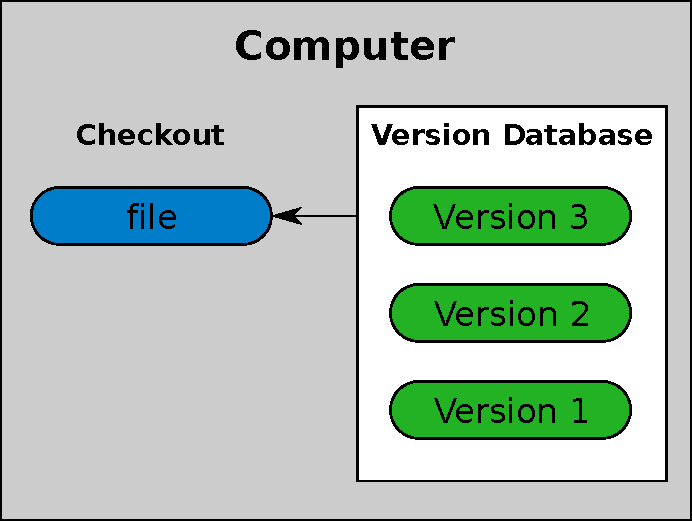
\includegraphics[height=.5\textheight]{own_fig/vc_single}  

\begin{columns}
\column{.2\textwidth}

\column{.8\textwidth}
\begin{description}[version database]
 \item[checkout] working directory
 \item[version database] repository
\end{description}

\end{columns}
  
\end{frame}

% -------------------------------------

\begin{frame}{Version Control: Central}
\centering
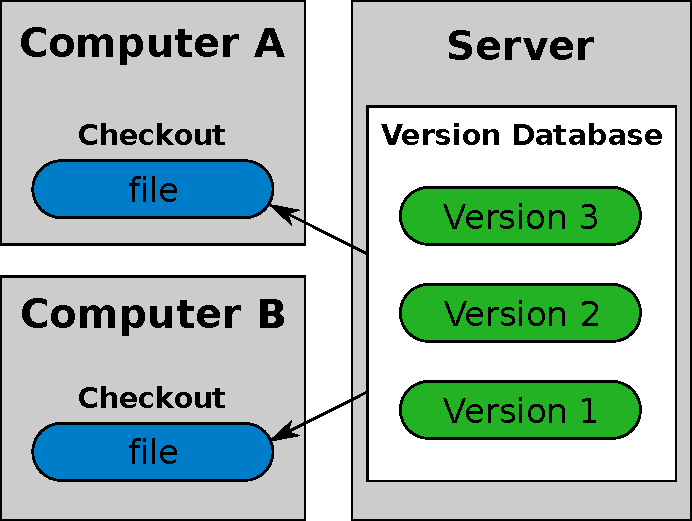
\includegraphics[height=.5\textheight]{own_fig/vc_central}

\end{frame}

% -------------------------------------

\begin{frame}{Version Control: Distributed}
\centering
  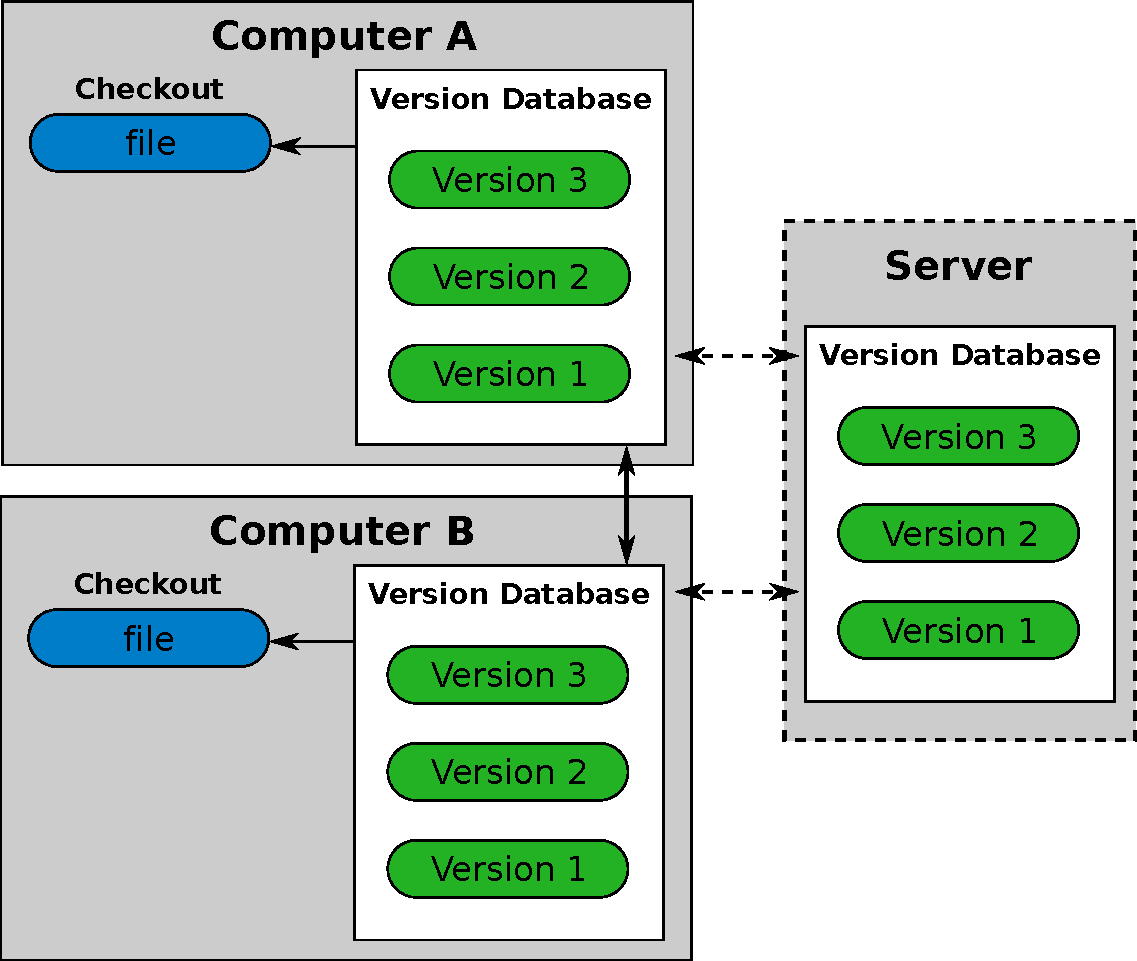
\includegraphics[height=0.8\textheight]{own_fig/vc_distributed}
\end{frame}

% -------------------------------------

\begin{frame}[fragile]{\git: Help}
\footnotesize
\begin{verbatim}
usage: git [OPTIONS] COMMAND [ARGS]

The most commonly used git commands are:
   add        Add file contents to the index
   commit     Record changes to the repository
   diff       Show changes between commits, commit and working tree, etc
   ...



git help <command>
git help <concept>  

git status

\end{verbatim}
\end{frame}

% -------------------------------------

\begin{frame}{\git: Introduce yourself}
  \begin{center}
    \small
    \texttt{git config -{}-global user.name "Nicola Chiapolini"}
  \end{center}
  \vspace{0.2cm}
  \begin{center}
    \small
    \texttt{git config -{}-global user.email "nchiapol@physik.uzh.ch"}
  \end{center}
\end{frame}

% -------------------------------------

\section[Single+Local]{Single developer + local repository}
\againframe<3>{outline}

% -------------------------------------

% \begin{frame}{Single+Local \git: Motivations}
%   \begin{itemize}
%   \item Why VC for single developer + local repository?
%     \begin{itemize}
%     \item First step towards a shared project.
%     \item Backup.
%     \item To keep the memory of your work.
%     \end{itemize}
%   \end{itemize}
% \end{frame}

% -------------------------------------

\begin{frame}{Single+Local \git: Init}
  \begin{center}
    \texttt{git init}
  \end{center}
  \begin{itemize}
  \item Creates an empty \git repository.
  \item Creates the git directory: \texttt{.git/}
  \end{itemize}
  \begin{figure}
    \centering
    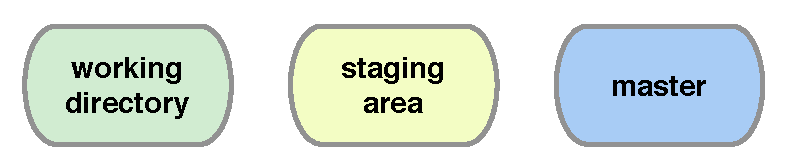
\includegraphics[width=0.75\textwidth]{figs/local-init}
  \end{figure}

\begin{itemize}
   \item<alert@2> does not change your files
\end{itemize}
\end{frame}

% -------------------------------------

\begin{frame}{Single+Local \git: Add}
  \begin{center}
    \texttt{git add file1 [file2 ...]}
  \end{center}
  \begin{itemize}
  \item Adds new files for next commit
  \item Adds content from working dir for next commit
  \item DOES NOT add info on file permissions other than \emph{exec/noexec}
  \item DOES NOT add directories \emph{per se}.
  \end{itemize}
  \begin{figure}
    \centering
    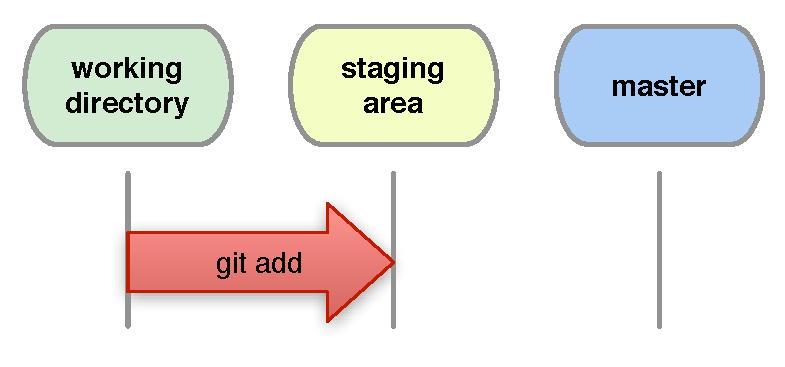
\includegraphics[width=0.75\textwidth]{figs/local-add}
  \end{figure}
\end{frame}

% -------------------------------------

\begin{frame}{Single+Local \git: Commit}
  \begin{center}
    \texttt{git commit [-m "Commit message."]}
  \end{center}
  Records changes from the staging area to master.
  \begin{figure}
    \centering
    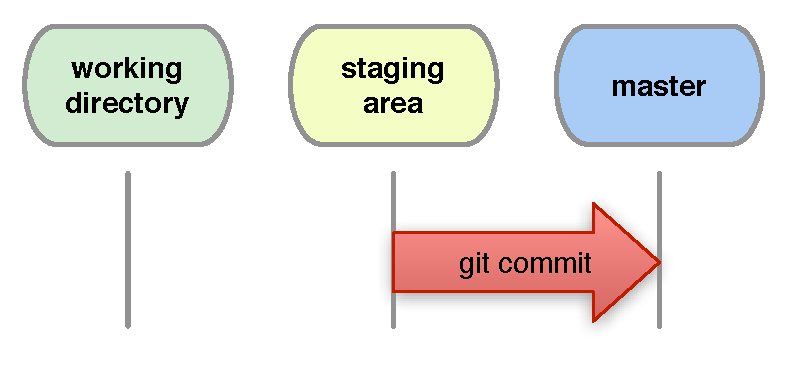
\includegraphics[width=0.75\textwidth]{figs/local-commit}
  \end{figure}
\end{frame}

% -------------------------------------

\begin{frame}{Single+Local \git: Direct Commit}
  \begin{center}
    \texttt{git commit file1 file2 [-m "Commit message."]}
  \end{center}
  Records all changes of \texttt{file1},
  \texttt{file2} from working dir and staging area to master.
  \begin{figure}
    \centering
    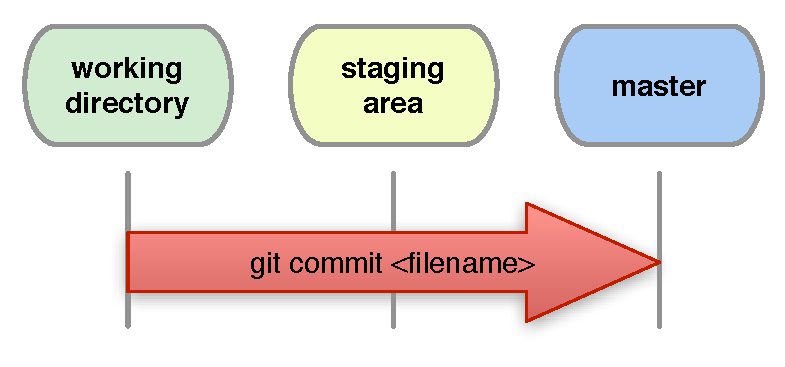
\includegraphics[width=0.75\textwidth]{figs/local-commit-filename}
  \end{figure}
  \begin{center}
    \texttt{git commit -a[m "Commit message."]}
  \end{center}
  Records all changes in working dir and staging area. \emph{Be Careful!}
\end{frame}

% -------------------------------------

\begin{frame}{Single+Local \git: Diff}
  \begin{center}
    \texttt{git diff [filename|...]}
  \end{center}
  Shows changes between \emph{working directory}\\
  and \emph{staging area}
  \begin{figure}
    \centering
    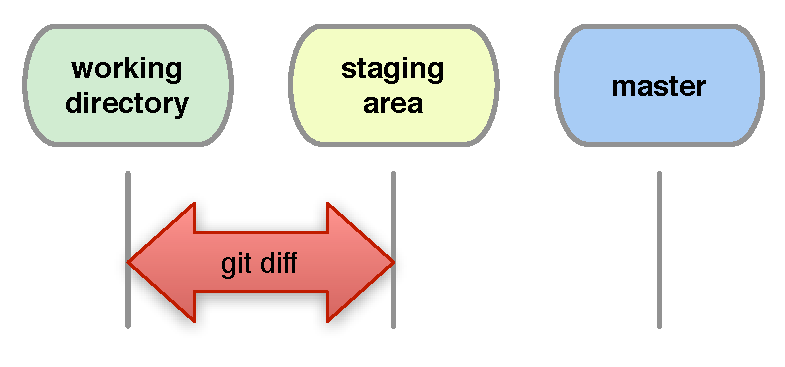
\includegraphics[width=0.75\textwidth]{figs/local-diff}
  \end{figure}
\end{frame}

% -------------------------------------

\begin{frame}{Single+Local \git: Diff Staged}
  \begin{block}{How do I see what is staged?}
    \texttt{git diff -{}-staged} shows differences\\ between
    staging area and last commit.
  \end{block}
  \begin{figure}
    \centering
    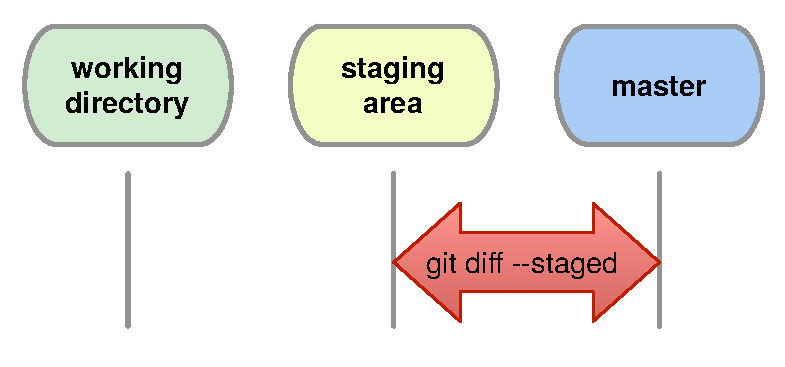
\includegraphics[width=0.75\textwidth]{own_fig/local-diff-staged}
  \end{figure}
\end{frame}

% -------------------------------------

\begin{frame}{Single+Local \git: Logs}
  \begin{center}
    \texttt{git log [-{}-oneline]}
  \end{center}
  Shows details of the commits.
  \begin{figure}
    \centering
    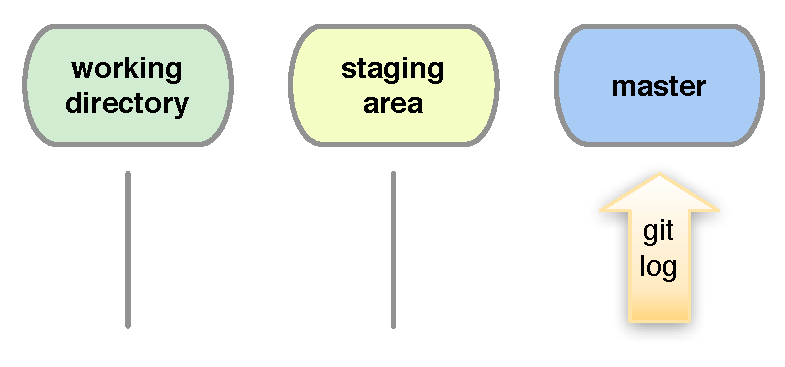
\includegraphics[width=0.75\textwidth]{figs/local-log}
  \end{figure}
\end{frame}

% -------------------------------------

\begin{frame}{Single+Local \git: Graphic Logs}
  \begin{center}
    \texttt{gitk} / \texttt{gitg}
  \end{center}
  GUI to browse the \git repository.
  \begin{figure}
    \centering
    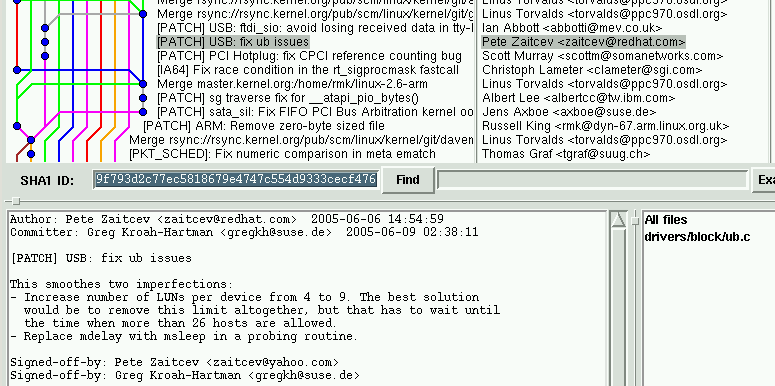
\includegraphics[width=0.8\textwidth]{figs/gitk_cropped}
  \end{figure}
\end{frame}

% -------------------------------------

\begin{frame}{Single+Local \git: Changing Version}
  \begin{center}
    \texttt{git checkout <file|commit>}
  \end{center}
  
  \begin{figure}
    \centering
    \includegraphics<1>[width=0.75\textwidth]{own_fig/local-checkout-file}
    \includegraphics<2>[width=0.75\textwidth]{own_fig/local-checkout-commit}
  \end{figure}
\end{frame}

% -------------------------------------

\begin{frame}{Single+Local \git: (Re)move.}
  \alert{Warning}: whenever you want to \emph{remove}, \emph{move} or
  \emph{rename} a tracked file use \git:
  \begin{center}
    \texttt{\textbf{git rm <filename>}}
  \end{center}
  \begin{center}
    \texttt{\textbf{git mv <oldname> <newname>}}
  \end{center}
Remember to \texttt{\textbf{commit}} these changes!
  \begin{center}
    \texttt{\textbf{git commit -m "File (re)moved."}}
  \end{center}
\end{frame}

% -------------------------------------

\subsection{Demo/Exercise: Single+Local}
\againframe<4>{outline}

% -------------------------------------

\section[multi+remote/shared]{Multiple developers + remote central repository}
\againframe<5>{outline}

% -------------------------------------

\begin{frame}{multi+remote/shared \git: Setup}
  \begin{figure}
    \centering
    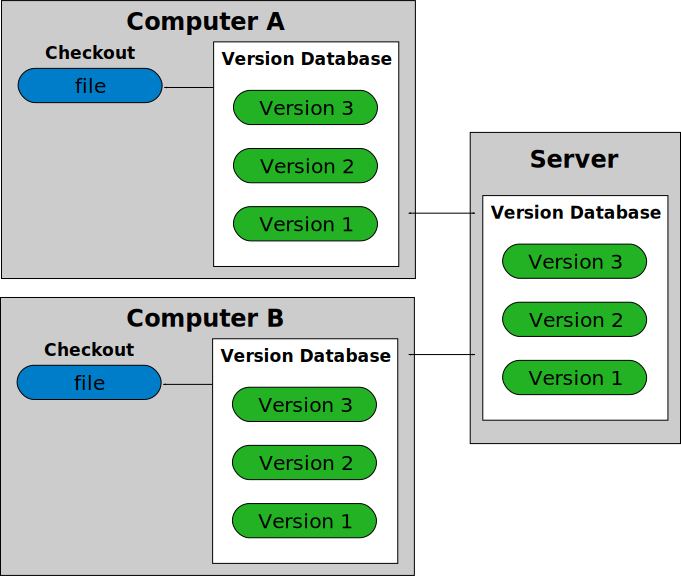
\includegraphics[height=0.8\textheight]{own_fig/vc_central-git}
  \end{figure}
\end{frame}

% -------------------------------------

\begin{frame}{multi+remote/shared \git: Clone}
  \begin{center}
    \texttt{\textbf{git clone <URL>}}
  \end{center}
  \uncover<2->{Creates \alert{two} local copies of the 
    \alert{whole} remote repository.}
  \begin{figure}
    \begin{center}
      \includegraphics<1>[width=9cm]{own_fig/local-remote_clone-1}
      \includegraphics<2>[width=9cm]{own_fig/local-remote_clone-2}
    \end{center}
  \end{figure}
  \begin{block}<2->{Hint}
    \texttt{git remote -v} \hspace{0.5cm} shows \textbf{name} and \texttt{URL} of the remote repository.
  \end{block}
\end{frame}

% -------------------------------------

\begin{frame}{multi+remote/shared \git: Commands}
  \begin{figure}
    \centering
    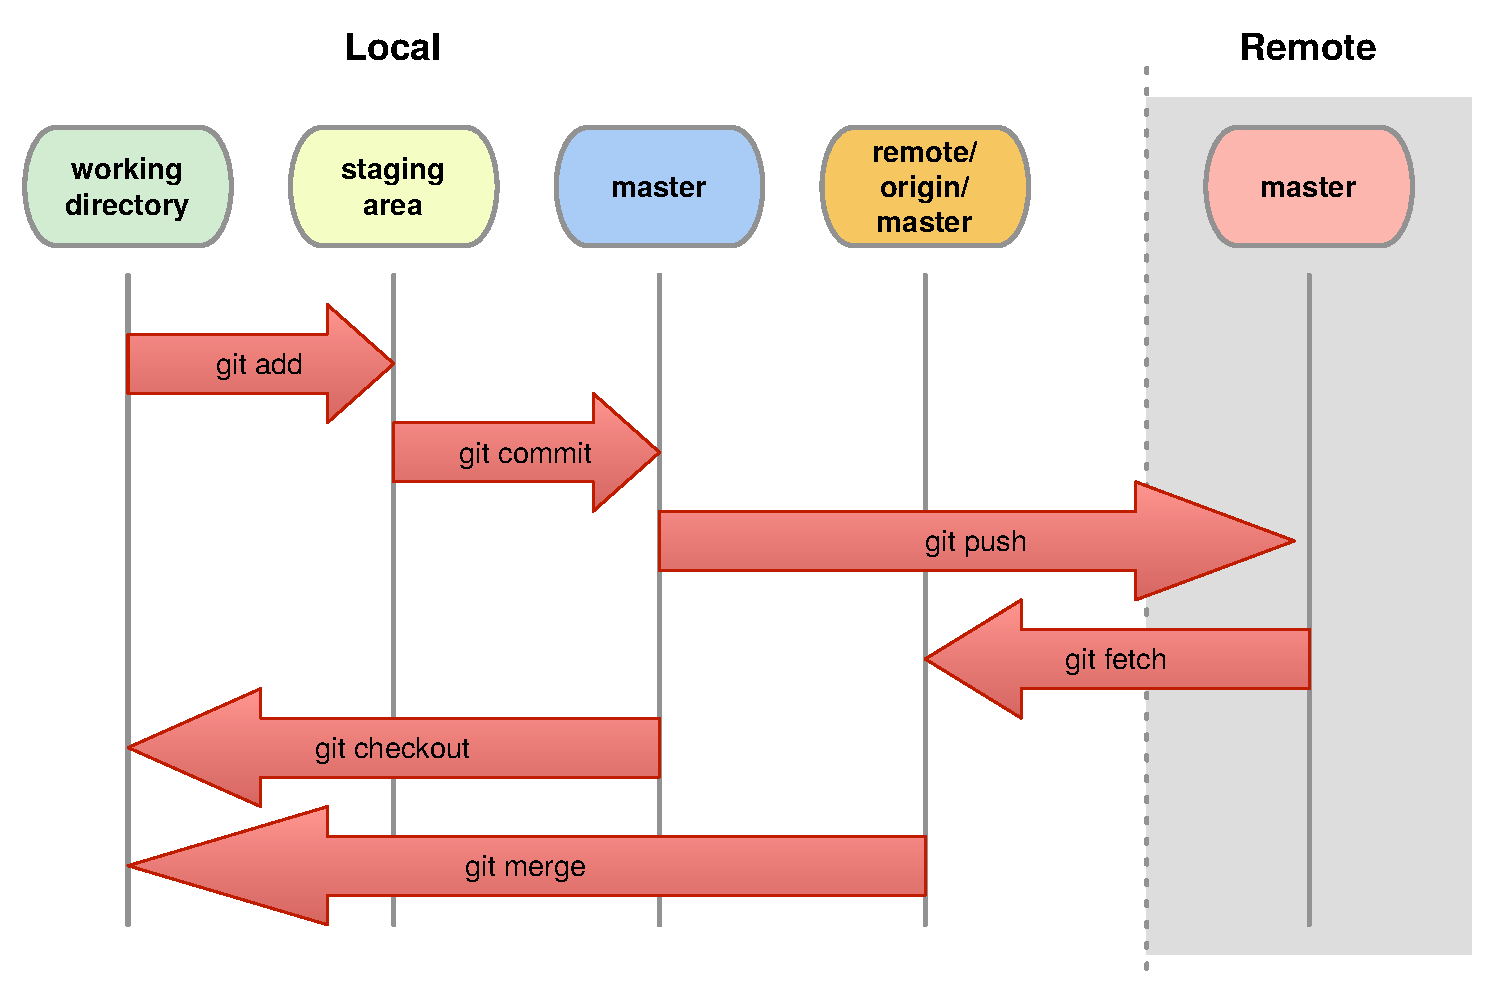
\includegraphics[height=0.8\textheight]{own_fig/local-remote}
  \end{figure}  
\end{frame}

% -------------------------------------

\begin{frame}{multi+remote/shared \git: Fetch}
  \begin{center}
    \texttt{\textbf{git fetch}}
  \end{center}
  \begin{itemize}
  \item Updates origin master from remote master
  \item local master, staging area and working dir not changed
  \end{itemize}
  \begin{figure}
    \centering
    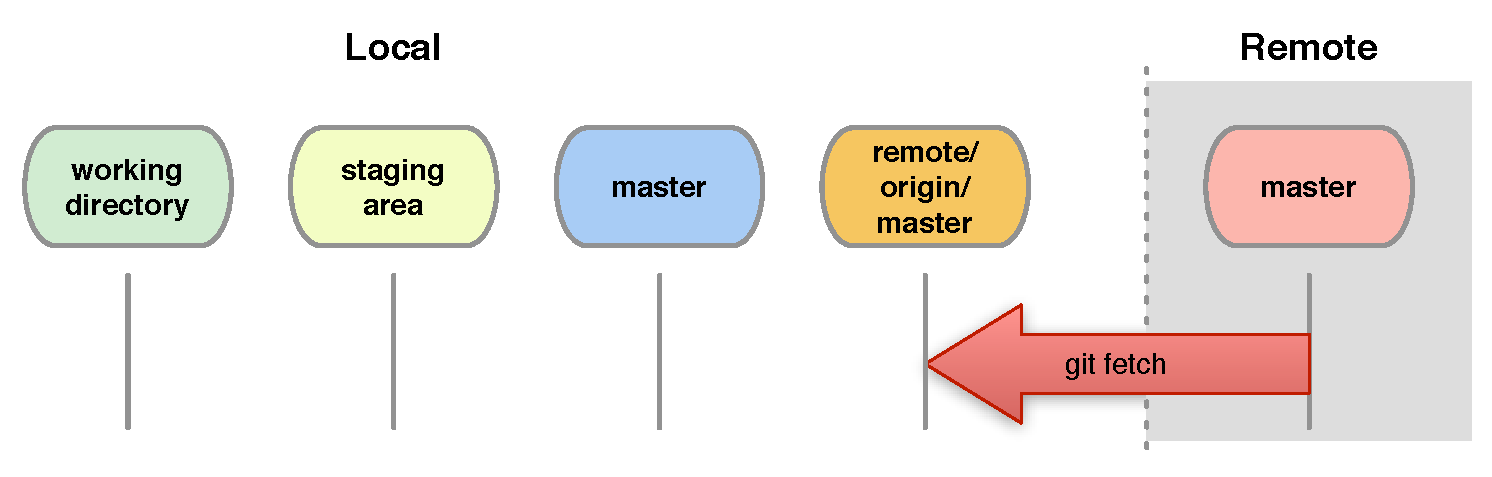
\includegraphics[width=9.5cm]{figs/local-remote-fetch}
  \end{figure}
\end{frame}

% -------------------------------------

\begin{frame}{multi+remote/shared \git: Merge}
  \begin{center}
    \texttt{\textbf{git merge}}
  \end{center}
  \begin{itemize}
  \item combines changes from both sources
  \item \alert{Warning}: can generate \emph{conflicts}!
  \end{itemize}
  \begin{figure}
    \centering
    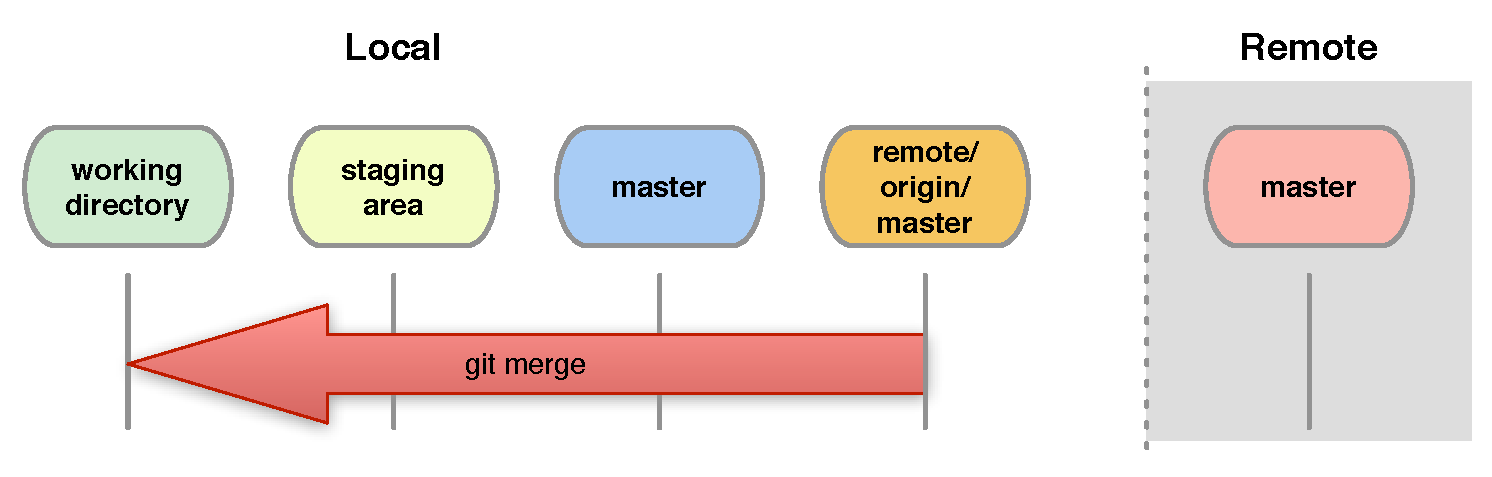
\includegraphics[width=9.5cm]{figs/local-remote-merge}
  \end{figure}
  \begin{center}
    \texttt{\textbf{git fetch}} + \texttt{\textbf{git merge}} = \texttt{\textbf{git pull}}
  \end{center}
\end{frame}

% -------------------------------------

\begin{frame}[fragile]{multi+remote/shared \git: Conflicts}
  \begin{center}
    \alert{Conflict!}
  \end{center}
\begin{verbatim}
  ...
  <<<<<<< yours:sample.txt
  Conflict resolution is hard;
  let's go shopping.
  =======
  Git makes conflict resolution easy.
  >>>>>>> theirs:sample.txt
  ...
\end{verbatim}
\end{frame}

% -------------------------------------

\begin{frame}{multi+remote/shared \git: Resolving Conflicts}
\begin{enumerate}
\item See where conflicts are:
  \begin{center}
  \texttt{git diff}
  \end{center}
\item Edit conflicting lines.
\item Add changes to the staging area:
  \begin{center}
    \texttt{git add file1 [...]}
  \end{center}
\item Commit changes:
  \begin{center}
    \texttt{git commit -m "Conflicts solved."}
  \end{center}
\end{enumerate}
\end{frame}

% -------------------------------------

\begin{frame}{multi+remote/shared \git: Push}
  \begin{center}
    \texttt{\textbf{git push}}
  \end{center}
  \begin{itemize}
  \item Updates \emph{remote master}.
  \item Requires \texttt{\textbf{fetch}}+\texttt{\textbf{merge}} first.
  \end{itemize}
  \begin{figure}
    \centering
    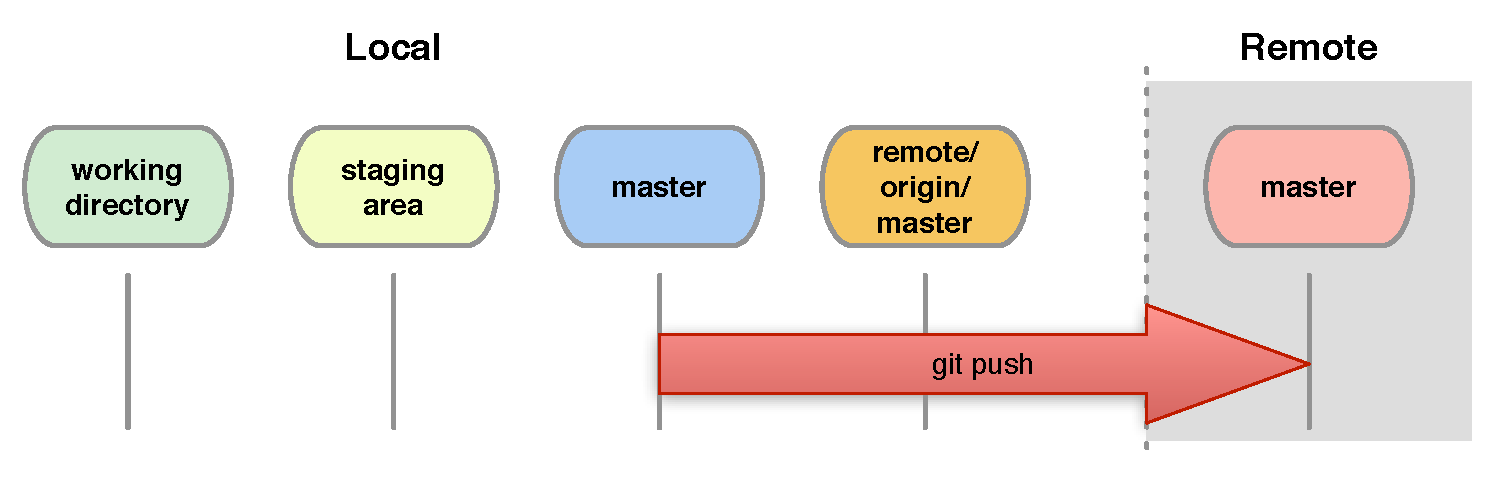
\includegraphics[width=9.5cm]{figs/local-remote-push}
  \end{figure}
\end{frame}

% -------------------------------------

\subsection{Demo/Exercise: Multi+Remote/Shared}
\againframe<6>{outline}

% -------------------------------------

\begin{frame}{Setting up a remote+shared repository. }
  Share repository via \texttt{\textbf{ssh}}
  \begin{block}{On \emph{remote} server create
      \textbf{bare}+\textbf{shared} repository:}
    \begin{itemize}
    \item \texttt{\textbf{mkdir newproject}}
    \item set up proper \emph{group} permissions: \texttt{\textbf{chmod g+rw\alert{s} newproject}}
    \item \texttt{\textbf{cd newproject}}
    \item \texttt{\textbf{git \alert{-{}-bare} init \alert{-{}-shared=group}}}
    \end{itemize}
  \end{block}
  Everybody clones: \texttt{\textbf{git clone ssh://remote.com/path/newproject}}
\end{frame}

% -------------------------------------

\section{Behind the Scenes}
\againframe<7>{outline}

% -------------------------------------

\begin{frame}<1-11,15->[fragile, label=behindthescenes]
  \frametitle<1-4,15>{Behind the Scenes: Setup}
  \frametitle<5-11>{Behind the Scenes: Branches}
  \frametitle<12-14>{Behind the Scenes: Rebase}
  \def\develmax{13}
  \def\mastermax{14}
  \frametitle<16-17>{Behind the Scenes: Tags}
  \frametitle<18->{Behind the Scenes: Detached HEAD}

%% debug output, printing the slide number
% this is slide \arabic{slideinframe}

\def\xshift{2cm}
\def\yshift{1cm}
\def\ccol{black}
\def\bcol{green}
\def\hcol{brown}
\def\tcol{orange}

% add the head label offset in x; Arguments: slide_nr, node_name
\newcommand{\head}[1]{
\only<\sid>{
\node (head) [head, xshift=\xshift] at (#1) { HEAD };
\draw [harrow] (head) edge (#1);
}
}
% add the head label offset in y; Arguments: slide_nr, node_name
\newcommand{\heady}[1]{
\only<\sid>{
\node (head) [head, yshift=\yshift] at (#1) { HEAD };
\draw [harrow] (head) edge (#1);
}
}
% add the master label; Arguments: slide_nr, node_name
\newcommand{\master}[1]{
\only<\sid>{
\node (master) [branch, yshift=-\yshift] at (#1) { master };
\draw [barrow] (master) edge (#1);
}
}
% add the devel label; Arguments: slide_nr, node_name
\newcommand{\devel}[1]{
\only<\sid>{
\node (devel) [branch, yshift=\yshift] at (#1) { devel };
\draw [barrow] (devel) edge (#1);
}
}
% add the master+head labels; Arguments: slide_nr, node_name
\newcommand{\masterhead}[1]{
\master{#1}
\head{master}
}
% add the devel+head labels; Arguments: slide_nr, node_name
\newcommand{\develhead}[1]{
\devel{#1}
\head{devel}
}
% print the git command we executed on top of the picture
\newcommand{\gitcmd}[1]{
\only<\sid>{
\node (gitcmd) [xshift=2.3*\xshift, yshift=3*\yshift, align=center] at (a) { \texttt{#1} };
}
}

\newcount\sid
\sid 1 
\newcommand{\next}{\advance\sid by 1 }
\begin{tikzpicture}
\tikzstyle{commit}=[inner sep=.5em, draw=\ccol!30, thick, fill=\ccol!10, rounded corners];
\tikzstyle{carrow}=[\ccol, -Stealth];
\tikzstyle{branch}=[inner sep=.5em, draw=\bcol!30, thick, fill=\bcol!10, sharp corners];
\tikzstyle{barrow}=[\bcol, -Stealth];
\tikzstyle{head}=[inner sep=.5em, draw=\hcol!30, thick, fill=\hcol!10, sharp corners];
\tikzstyle{harrow}=[\hcol, -Stealth];
\tikzstyle{tag}=[inner sep=.5em, draw=\tcol!50, thick, fill=\tcol!20, sharp corners];
\tikzstyle{tarrow}=[\tcol, -Stealth];

\node (a) [commit] {a};
\gitcmd{git init; git add [...]; git commit -m "A: init"}
\node (topright)    [xshift=6*\xshift,yshift=3.3*\yshift]  at (a) {};
\node (bottomright) [xshift=6*\xshift,yshift=-1.5*\yshift] at (a) {};
\node (leftedge)    [xshift=-0.5*\xshift] at (a) {};

\next 
\gitcmd{git init; git add [...]; git commit -m "A: init"}
\masterhead{a}


\next 
\gitcmd{git commit -am "B"}
\only<\sid->{
\node (b) [commit, xshift=\xshift] at (a) { b };
\draw [carrow] (b) edge (a);
}
\masterhead{b}

\next 
\gitcmd{git commit -am "C"}
\only<\sid->{
\node (c) [commit, xshift=\xshift] at (b) { c };
\draw [carrow] (c) edge (b);
}
\masterhead{c}

\next
\gitcmd{git branch devel}
\masterhead{c}
\devel{c}

\next
\gitcmd{git checkout devel}
\master{c}
\develhead{c}

\next
\gitcmd{git commit -am "D"}
\only<\sid-\develmax>{
\node (d) [commit, yshift=\yshift] at (c) { d };
\draw [carrow] (d) edge (c);
}
\master{c}
\develhead{d}

\next
\gitcmd{git commit -am "E"}
\only<\sid-\develmax>{
\node (e) [commit, xshift=\xshift] at (d) { e };
\draw [carrow] (e) edge (d);
}
\master{c}
\develhead{e}

\next
\gitcmd{git checkout master}
\masterhead{c}
\devel{e}

\next
\gitcmd{git commit -am "F"}
\only<\sid-\mastermax>{
\node (f) [commit, xshift=\xshift] at (c) { f };
\draw [carrow] (f) edge (c);
}
\masterhead{f}
\devel{e}

\next
\gitcmd{git merge devel}
\only<\sid>{
\node (g) [commit, xshift=\xshift] at (f) { g };
\draw [carrow] (g) edge (f);
\draw [carrow] (g) edge (e);
}
\masterhead{g}
\devel{e}

\next
\gitcmd{git commit -am "F"}
\masterhead{f}
\devel{e}

\next
\gitcmd{git checkout devel}
\master{f}
\develhead{e}

\next
\gitcmd{git rebase master}
\only<\sid>{
\node (d) [commit, yshift=\yshift] at (f) { d' };
\draw [carrow] (d) edge (f);
}
\only<\sid>{
\node (e) [commit, xshift=\xshift] at (d) { e' };
\draw [carrow] (e) edge (d);
}
\master{f}
\develhead{e}

\next
\gitcmd{git commit -am "C"}
\masterhead{c}

\next
\gitcmd{git tag v1.0}
\only<\sid->{
\node (vers) [tag, yshift=-\yshift] at (b) { v1.0 };
\draw [tarrow] (vers) edge (c);
}
\masterhead{c}

\next
\gitcmd{git commit -am "H"}
\only<\sid->{
\node (h) [commit, xshift=\xshift] at (c) { h };
\draw [carrow] (h) edge (c);
}
\masterhead{h}

\next
\gitcmd{git checkout b}
\master{h}
\heady{b}

\next
\gitcmd{git commit -am "J"}
\only<\sid->{
\node (j) [commit, yshift=\yshift] at (b) { j };
\draw [carrow] (j) edge (b);
}
\master{h}
\heady{j}

\next
\gitcmd{git commit -am "K"}
\only<\sid->{
\node (k) [commit, xshift=\xshift] at (j) { k };
\draw [carrow] (k) edge (j);
}
\master{h}
\heady{k}

\next
\gitcmd{git checkout master}
\masterhead{h}

\next
\gitcmd{git commit -am "K"}
\master{h}
\heady{k}

\next
\gitcmd{git checkout -b devel}
\master{h}
\develhead{k}

\next
\gitcmd{git checkout master}
\masterhead{h}
\devel{k}

\end{tikzpicture}

\def\xshift{3cm}
\def\yshift{0.8cm}
\begin{tikzpicture}
\tikzstyle{wd}=[inner sep=.5em, draw=black!30, thick, fill=green!30, rounded corners];
\tikzstyle{sa}=[inner sep=.5em, draw=black!30, thick, fill=yellow!30, rounded corners];
\tikzstyle{rep}=[inner sep=.5em, draw=black!30, thick, fill=blue!30, rounded corners];

\node (master) [rep] {master};
\node (topright)    [xshift=-3*\xshift, yshift=0.5*\yshift]  at (master) {};
\node (bottomright) [xshift=-3*\xshift, yshift=-1.7*\yshift] at (master) {};

\only<1-5,9-12,15-17,21,24>{
  \node (sa) [xshift=-\xshift, sa] at (master) {staging area};
  \node (wd) [xshift=-\xshift, wd] at (sa) { working dir };
}
\only<5-14,23->{\node (devel) [yshift=-\yshift, rep] at (master) {devel};}
\only<6-8,13-14,23>{
  \node (sa) [xshift=-\xshift, sa] at (devel) {staging area};
  \node (wd) [xshift=-\xshift, wd] at (sa) { working dir };
}
\only<18-20,22>{
  \node (sa) [xshift=-\xshift, yshift=-\yshift, sa] at (master) {staging area};
  \node (wd) [xshift=-\xshift, wd] at (sa) { working dir };
}

\end{tikzpicture}
\end{frame}

% -------------------------------------

% \section{Questions}
% \againframe<7>{outline}

% -------------------------------------

\begin{frame}{}
  
  {\centering \LARGE \alert{Questions?}
  
  }
  \vspace*{8mm}
  Understanding how \git works:
  \begin{itemize}
  \item \git foundations, by Matthew Brett:
    \small
    \url{http://matthew-brett.github.com/pydagogue/foundation.html}
  \item  The \git parable, by Tom Preston-Werner:
    \small
  \url{http://tom.preston-werner.com/2009/05/19/the-git-parable.html}
  \end{itemize}
  \vspace*{1em}
  Excellent guides:
  \begin{itemize}
  \item ``Pro Git'' book: \url{http://git-scm.com/book} (FREE)
  \item \git magic: \url{http://www-cs-students.stanford.edu/~blynn/gitmagic/}
  \end{itemize}
\end{frame}

% -------------------------------------

\appendix

\againframe<13-14>{behindthescenes}


\end{document}
